\documentclass[border=2pt]{standalone}
\usepackage{tikz}
\usetikzlibrary{calc} \usetikzlibrary{positioning} \usetikzlibrary{shapes,arrows} \usetikzlibrary{plotmarks}
\usepackage{pgfplots}
\usetikzlibrary{patterns}

\begin{document}

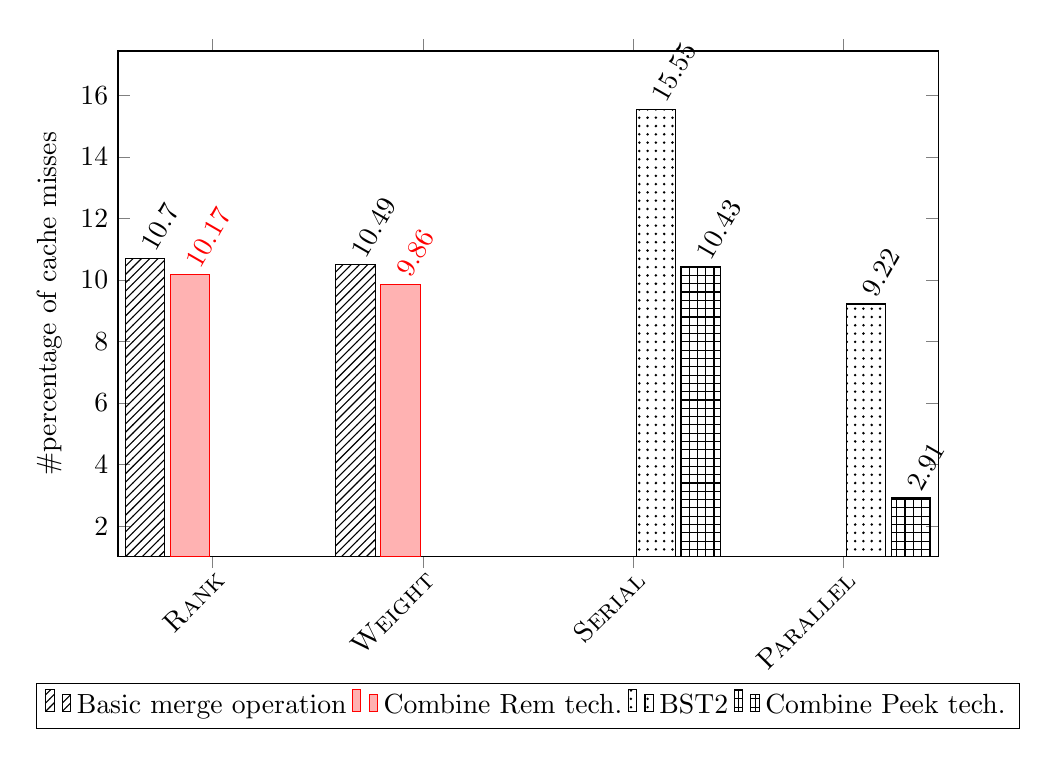
\begin{tikzpicture}
  \centering
  \begin{axis}[
  	bar width=0.5cm,
    ybar,
    xtick=\empty,
    enlargelimits=0.15,
    legend style={at={(0.5,-0.25)},
    anchor=north,legend columns=-2},
    ylabel={\#percentage of cache misses},
    symbolic x coords={Rank,Weight,Serial,Parallel},
    xtick={Rank,Weight,Serial,Parallel},
    height=8cm,width=12cm,
    nodes near coords,
    nodes near coords align={vertical},
    every node near coord/.append style={
        anchor=mid west,
        rotate=60
    },
    xticklabel style={
	    inner sep=0pt,
	    anchor=north east,
	    rotate=45,
	    font=\scshape,
    },
    % enlarge y limits={upper,value=0.3},
    ]
    \addplot[pattern=north east lines] coordinates {(Rank,10.701) (Weight,10.491)};
    \addplot coordinates {(Rank,10.167) (Weight,9.856)};
    \addplot[pattern=dots] coordinates {(Serial,15.546)  (Parallel,9.218)};
    \addplot[pattern=grid] coordinates {(Serial,10.430)  (Parallel,2.914)};
    \legend{Basic merge operation, Combine Rem tech., BST2, Combine Peek tech.};
  \end{axis}
\end{tikzpicture}


\end{document}
